\documentclass[twoside]{book}

% Packages required by doxygen
\usepackage{fixltx2e}
\usepackage{calc}
\usepackage{doxygen}
\usepackage[export]{adjustbox} % also loads graphicx
\usepackage{graphicx}
\usepackage[utf8]{inputenc}
\usepackage{makeidx}
\usepackage{multicol}
\usepackage{multirow}
\PassOptionsToPackage{warn}{textcomp}
\usepackage{textcomp}
\usepackage[nointegrals]{wasysym}
\usepackage[table]{xcolor}

% Font selection
\usepackage[T1]{fontenc}
\usepackage[scaled=.90]{helvet}
\usepackage{courier}
\usepackage{amssymb}
\usepackage{sectsty}
\renewcommand{\familydefault}{\sfdefault}
\allsectionsfont{%
  \fontseries{bc}\selectfont%
  \color{darkgray}%
}
\renewcommand{\DoxyLabelFont}{%
  \fontseries{bc}\selectfont%
  \color{darkgray}%
}
\newcommand{\+}{\discretionary{\mbox{\scriptsize$\hookleftarrow$}}{}{}}

% Page & text layout
\usepackage{geometry}
\geometry{%
  a4paper,%
  top=2.5cm,%
  bottom=2.5cm,%
  left=2.5cm,%
  right=2.5cm%
}
\tolerance=750
\hfuzz=15pt
\hbadness=750
\setlength{\emergencystretch}{15pt}
\setlength{\parindent}{0cm}
\setlength{\parskip}{3ex plus 2ex minus 2ex}
\makeatletter
\renewcommand{\paragraph}{%
  \@startsection{paragraph}{4}{0ex}{-1.0ex}{1.0ex}{%
    \normalfont\normalsize\bfseries\SS@parafont%
  }%
}
\renewcommand{\subparagraph}{%
  \@startsection{subparagraph}{5}{0ex}{-1.0ex}{1.0ex}{%
    \normalfont\normalsize\bfseries\SS@subparafont%
  }%
}
\makeatother

% Headers & footers
\usepackage{fancyhdr}
\pagestyle{fancyplain}
\fancyhead[LE]{\fancyplain{}{\bfseries\thepage}}
\fancyhead[CE]{\fancyplain{}{}}
\fancyhead[RE]{\fancyplain{}{\bfseries\leftmark}}
\fancyhead[LO]{\fancyplain{}{\bfseries\rightmark}}
\fancyhead[CO]{\fancyplain{}{}}
\fancyhead[RO]{\fancyplain{}{\bfseries\thepage}}
\fancyfoot[LE]{\fancyplain{}{}}
\fancyfoot[CE]{\fancyplain{}{}}
\fancyfoot[RE]{\fancyplain{}{\bfseries\scriptsize Generated by Doxygen }}
\fancyfoot[LO]{\fancyplain{}{\bfseries\scriptsize Generated by Doxygen }}
\fancyfoot[CO]{\fancyplain{}{}}
\fancyfoot[RO]{\fancyplain{}{}}
\renewcommand{\footrulewidth}{0.4pt}
\renewcommand{\chaptermark}[1]{%
  \markboth{#1}{}%
}
\renewcommand{\sectionmark}[1]{%
  \markright{\thesection\ #1}%
}

% Indices & bibliography
\usepackage{natbib}
\usepackage[titles]{tocloft}
\setcounter{tocdepth}{3}
\setcounter{secnumdepth}{5}
\makeindex

% Hyperlinks (required, but should be loaded last)
\usepackage{ifpdf}
\ifpdf
  \usepackage[pdftex,pagebackref=true]{hyperref}
\else
  \usepackage[ps2pdf,pagebackref=true]{hyperref}
\fi
\hypersetup{%
  colorlinks=true,%
  linkcolor=blue,%
  citecolor=blue,%
  unicode%
}

% Custom commands
\newcommand{\clearemptydoublepage}{%
  \newpage{\pagestyle{empty}\cleardoublepage}%
}

\usepackage{caption}
\captionsetup{labelsep=space,justification=centering,font={bf},singlelinecheck=off,skip=4pt,position=top}

%===== C O N T E N T S =====

\begin{document}

% Titlepage & ToC
\hypersetup{pageanchor=false,
             bookmarksnumbered=true,
             pdfencoding=unicode
            }
\pagenumbering{roman}
\begin{titlepage}
\vspace*{7cm}
\begin{center}%
{\Large Tiny\+Str }\\
\vspace*{1cm}
{\large Generated by Doxygen 1.8.11}\\
\end{center}
\end{titlepage}
\clearemptydoublepage
\tableofcontents
\clearemptydoublepage
\pagenumbering{arabic}
\hypersetup{pageanchor=true}

%--- Begin generated contents ---
\chapter{Tiny\+Str}
\label{index}\hypertarget{index}{}See \hyperlink{tinystr_8h}{tinystr.\+h} 
\chapter{Overview}
\label{md_Readme}
\hypertarget{md_Readme}{}
\hyperlink{unionTinyStr}{Tiny\+Str} is a C library for efficiently dealing with short strings (7 characters at most).

Internally strings are stored as a union between a character array with 8 elements and a 64-\/bit integer, using bitwise operations on the latter where possible for speed. They are always null terminated and additionally they have the property that any bytes beyond the first null byte, are also null bytes, giving each string a unique representation.

\subsubsection*{Compiling and Using}

See the included {\ttfamily Makefile} and {\ttfamily example.\+c} source file.

\subsubsection*{Operations}

\tabulinesep=1mm
\begin{longtabu} spread 0pt [c]{*3{|X[-1]}|}
\hline
\rowcolor{\tableheadbgcolor}{\bf Operation }&{\bf Prototype }&{\bf Notes  }\\\cline{1-3}
\endfirsthead
\hline
\endfoot
\hline
\rowcolor{\tableheadbgcolor}{\bf Operation }&{\bf Prototype }&{\bf Notes  }\\\cline{1-3}
\endhead
Create New &\hyperlink{unionTinyStr}{Tiny\+Str} \hyperlink{tinystr_8h_a1014e8511651b9a255b42c42176d06b3}{tiny\+Str\+New(void)} &Returns empty string \\\cline{1-3}
Create From C-\/string &\hyperlink{unionTinyStr}{Tiny\+Str} \hyperlink{tinystr_8h_a180f5fb2d869a29a84e1bef615b5d7aa}{tiny\+Str\+From\+C(const char $\ast$cstr)} &Only at most the first 7 characters are copied. \\\cline{1-3}
Get Length &unsigned \hyperlink{tinystr_8h_af7822bd0caacdc85637c72281d72aabf}{tiny\+Str\+Len(\+Tiny\+Str str)} &\\\cline{1-3}
Test Equality &bool \hyperlink{tinystr_8h_a162f47ec690bcb03b097063d4d4fd605}{tiny\+Str\+Equal(\+Tiny\+Str str1, Tiny\+Str str2)} &\\\cline{1-3}
Compare &int tiny\+Str\+Cmp(\+Tiny\+Str str1, Tiny\+Str str2) &Acts as strcmp \\\cline{1-3}
Hash &uint64\+\_\+t \hyperlink{tinystr_8h_a083ff5929310b5b861aa520f8e93e92c}{tiny\+Str\+Perfect\+Hash(\+Tiny\+Str str)} &Returns a unique 64 bit integer for each valid string. \\\cline{1-3}
Hash (order perserving) &uint64\+\_\+t \hyperlink{tinystr_8h_a74aa53d4d62f156e9d954f39d5b519d3}{tiny\+Str\+Perfect\+Hash\+Order\+Preserving(\+Tiny\+Str str)} &Same as the above but if a$<$b (asciibetically) then f(a)$<$f(b), for all valid strings a and b. \\\cline{1-3}
Sub-\/string &\hyperlink{unionTinyStr}{Tiny\+Str} \hyperlink{tinystr_8h_ac1d49fc76dcbac990a6339b5a8f34056}{tiny\+Str\+Sub(\+Tiny\+Str str, unsigned offset, unsigned length)} &\\\cline{1-3}
Concatenate &\hyperlink{unionTinyStr}{Tiny\+Str} \hyperlink{tinystr_8h_a5df3565241f3d3b8a9ff37648648eeeb}{tiny\+Str\+Cat(\+Tiny\+Str str1, Tiny\+Str str2)} &\\\cline{1-3}
Truncate &\hyperlink{unionTinyStr}{Tiny\+Str} \hyperlink{tinystr_8h_a9e68ecf658de66bd7fd934035db9ae3d}{tiny\+Str\+Truncate(\+Tiny\+Str str, unsigned length)} &\\\cline{1-3}
printf &\hyperlink{unionTinyStr}{Tiny\+Str} tiny\+Str\+Printf(const char $\ast$format, ...) &See vprintf \\\cline{1-3}
vprintf &\hyperlink{unionTinyStr}{Tiny\+Str} \hyperlink{tinystr_8h_a91962a306055db78687958e848419e41}{tiny\+Str\+V\+Printf(const char $\ast$format, va\+\_\+list ap)} &Uses stdlib vsnprintf so acts identically. \\\cline{1-3}
Check Validity &bool \hyperlink{tinystr_8h_a7eda70f2f559a0f8c705c0f46c4ab105}{tiny\+Str\+Is\+Valid(\+Tiny\+Str str)} &As all unused bytes have to be null only a subset of all possible states are valid. \\\cline{1-3}
\end{longtabu}
Note\+: almost all functions are constant time, such as tiny\+Str\+Len, tiny\+Str\+Cat and tiny\+Str\+Cmp.

There is also a macro -\/ tiny\+Str\+ToC -\/ which gives a safe way to use a \hyperlink{unionTinyStr}{Tiny\+Str} as a const c-\/string.

\subsubsection*{Terms of use}

\hyperlink{unionTinyStr}{Tiny\+Str} is free, and distributed under the {\bfseries G\+NU General Public License} (G\+PL). Essentially, this means that you are free to do almost exactly what you want with the program, including distributing it among your friends, making it available for download from your web site, selling it (either by itself or as part of some bigger software package), or using it as the starting point for a software project of your own.

The only real limitation is that whenever you distribute \hyperlink{unionTinyStr}{Tiny\+Str} in some way, you must always include the full source code, or a pointer to where the source code can be found. If you make any changes to the source code, these changes must also be made available under the G\+PL.

For full details, read the copy of the G\+PL found in the file named {\itshape Copying.\+txt}. 
\chapter{Data Structure Index}
\section{Data Structures}
Here are the data structures with brief descriptions\+:\begin{DoxyCompactList}
\item\contentsline{section}{\hyperlink{unionTinyStr}{Tiny\+Str} }{\pageref{unionTinyStr}}{}
\end{DoxyCompactList}

\chapter{File Index}
\section{File List}
Here is a list of all documented files with brief descriptions\+:\begin{DoxyCompactList}
\item\contentsline{section}{\hyperlink{tinystr_8h}{tinystr.\+h} }{\pageref{tinystr_8h}}{}
\end{DoxyCompactList}

\chapter{Data Structure Documentation}
\hypertarget{unionTinyStr}{}\section{Tiny\+Str Union Reference}
\label{unionTinyStr}\index{Tiny\+Str@{Tiny\+Str}}
\subsection*{Data Fields}
\begin{DoxyCompactItemize}
\item 
uint64\+\_\+t {\bfseries integer}\hypertarget{unionTinyStr_ac7b6c2be68ebace734f0f39686d5f6ce}{}\label{unionTinyStr_ac7b6c2be68ebace734f0f39686d5f6ce}

\item 
char {\bfseries array} \mbox{[}8\mbox{]}\hypertarget{unionTinyStr_a90c27fcc65993dac2df7ba7451953f55}{}\label{unionTinyStr_a90c27fcc65993dac2df7ba7451953f55}

\end{DoxyCompactItemize}


The documentation for this union was generated from the following file\+:\begin{DoxyCompactItemize}
\item 
\hyperlink{tinystr_8h}{tinystr.\+h}\end{DoxyCompactItemize}

\chapter{File Documentation}
\hypertarget{tinystr_8h}{}\section{tinystr.\+h File Reference}
\label{tinystr_8h}\index{tinystr.\+h@{tinystr.\+h}}
{\ttfamily \#include $<$stdarg.\+h$>$}\\*
{\ttfamily \#include $<$stdbool.\+h$>$}\\*
{\ttfamily \#include $<$stdint.\+h$>$}\\*
Include dependency graph for tinystr.\+h\+:
\nopagebreak
\begin{figure}[H]
\begin{center}
\leavevmode
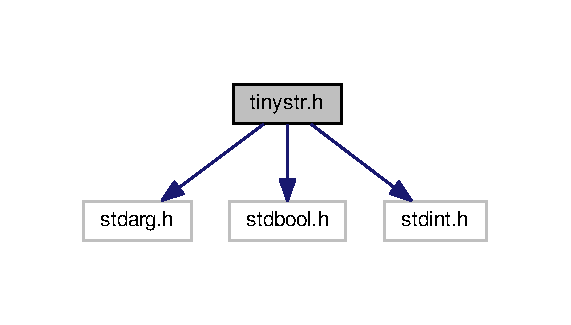
\includegraphics[width=274pt]{tinystr_8h__incl}
\end{center}
\end{figure}
\subsection*{Data Structures}
\begin{DoxyCompactItemize}
\item 
union \hyperlink{unionTinyStr}{Tiny\+Str}
\end{DoxyCompactItemize}
\subsection*{Macros}
\begin{DoxyCompactItemize}
\item 
\#define {\bfseries tiny\+Str\+ToC}(tiny\+Str)~((const char $\ast$)(tiny\+Str).array)\hypertarget{tinystr_8h_a663cb382e1a84995568daee2dff173aa}{}\label{tinystr_8h_a663cb382e1a84995568daee2dff173aa}

\end{DoxyCompactItemize}
\subsection*{Functions}
\begin{DoxyCompactItemize}
\item 
\hyperlink{unionTinyStr}{Tiny\+Str} \hyperlink{tinystr_8h_a5df3565241f3d3b8a9ff37648648eeeb}{tiny\+Str\+Cat} (\hyperlink{unionTinyStr}{Tiny\+Str} str1, \hyperlink{unionTinyStr}{Tiny\+Str} str2)
\item 
int {\bfseries tiny\+Str\+Cmp} (\hyperlink{unionTinyStr}{Tiny\+Str} str1, \hyperlink{unionTinyStr}{Tiny\+Str} str2)\hypertarget{tinystr_8h_ab712f6281ee326c4321ba0add729e943}{}\label{tinystr_8h_ab712f6281ee326c4321ba0add729e943}

\item 
bool \hyperlink{tinystr_8h_a162f47ec690bcb03b097063d4d4fd605}{tiny\+Str\+Equal} (\hyperlink{unionTinyStr}{Tiny\+Str} str1, \hyperlink{unionTinyStr}{Tiny\+Str} str2)
\item 
bool \hyperlink{tinystr_8h_a7eda70f2f559a0f8c705c0f46c4ab105}{tiny\+Str\+Is\+Valid} (\hyperlink{unionTinyStr}{Tiny\+Str} str)
\item 
\hyperlink{unionTinyStr}{Tiny\+Str} \hyperlink{tinystr_8h_a180f5fb2d869a29a84e1bef615b5d7aa}{tiny\+Str\+FromC} (const char $\ast$cstr)
\item 
unsigned \hyperlink{tinystr_8h_af7822bd0caacdc85637c72281d72aabf}{tiny\+Str\+Len} (\hyperlink{unionTinyStr}{Tiny\+Str} str)
\item 
\hyperlink{unionTinyStr}{Tiny\+Str} \hyperlink{tinystr_8h_a1014e8511651b9a255b42c42176d06b3}{tiny\+Str\+New} (void)
\item 
uint64\+\_\+t \hyperlink{tinystr_8h_a083ff5929310b5b861aa520f8e93e92c}{tiny\+Str\+Perfect\+Hash} (\hyperlink{unionTinyStr}{Tiny\+Str} str)
\item 
uint64\+\_\+t \hyperlink{tinystr_8h_a74aa53d4d62f156e9d954f39d5b519d3}{tiny\+Str\+Perfect\+Hash\+Order\+Preserving} (\hyperlink{unionTinyStr}{Tiny\+Str} str)
\item 
\hyperlink{unionTinyStr}{Tiny\+Str} \hyperlink{tinystr_8h_abcdfac7c9b279cc1708a66f5dd9d11c0}{tiny\+Str\+Printf} (const char $\ast$format,...)
\item 
\hyperlink{unionTinyStr}{Tiny\+Str} \hyperlink{tinystr_8h_ac1d49fc76dcbac990a6339b5a8f34056}{tiny\+Str\+Sub} (\hyperlink{unionTinyStr}{Tiny\+Str} str, unsigned offset, unsigned length)
\item 
\hyperlink{unionTinyStr}{Tiny\+Str} \hyperlink{tinystr_8h_a9e68ecf658de66bd7fd934035db9ae3d}{tiny\+Str\+Truncate} (\hyperlink{unionTinyStr}{Tiny\+Str} str, unsigned length)
\item 
\hyperlink{unionTinyStr}{Tiny\+Str} \hyperlink{tinystr_8h_a91962a306055db78687958e848419e41}{tiny\+Str\+V\+Printf} (const char $\ast$format, va\+\_\+list ap)
\end{DoxyCompactItemize}


\subsection{Function Documentation}
\index{tinystr.\+h@{tinystr.\+h}!tiny\+Str\+Cat@{tiny\+Str\+Cat}}
\index{tiny\+Str\+Cat@{tiny\+Str\+Cat}!tinystr.\+h@{tinystr.\+h}}
\subsubsection[{\texorpdfstring{tiny\+Str\+Cat(\+Tiny\+Str str1, Tiny\+Str str2)}{tinyStrCat(TinyStr str1, TinyStr str2)}}]{\setlength{\rightskip}{0pt plus 5cm}{\bf Tiny\+Str} tiny\+Str\+Cat (
\begin{DoxyParamCaption}
\item[{{\bf Tiny\+Str}}]{str1, }
\item[{{\bf Tiny\+Str}}]{str2}
\end{DoxyParamCaption}
)}\hypertarget{tinystr_8h_a5df3565241f3d3b8a9ff37648648eeeb}{}\label{tinystr_8h_a5df3565241f3d3b8a9ff37648648eeeb}
Append str2 to the end of str1 and return the reult. 
\begin{DoxyParams}{Parameters}
{\em str1} & first string \\
\hline
{\em str2} & second string \\
\hline
\end{DoxyParams}
\begin{DoxyReturn}{Returns}
combined string 
\end{DoxyReturn}
\index{tinystr.\+h@{tinystr.\+h}!tiny\+Str\+Equal@{tiny\+Str\+Equal}}
\index{tiny\+Str\+Equal@{tiny\+Str\+Equal}!tinystr.\+h@{tinystr.\+h}}
\subsubsection[{\texorpdfstring{tiny\+Str\+Equal(\+Tiny\+Str str1, Tiny\+Str str2)}{tinyStrEqual(TinyStr str1, TinyStr str2)}}]{\setlength{\rightskip}{0pt plus 5cm}bool tiny\+Str\+Equal (
\begin{DoxyParamCaption}
\item[{{\bf Tiny\+Str}}]{str1, }
\item[{{\bf Tiny\+Str}}]{str2}
\end{DoxyParamCaption}
)}\hypertarget{tinystr_8h_a162f47ec690bcb03b097063d4d4fd605}{}\label{tinystr_8h_a162f47ec690bcb03b097063d4d4fd605}
Compare two \hyperlink{unionTinyStr}{Tiny\+Str} objects for equality. 
\begin{DoxyParams}{Parameters}
{\em str1} & first string to compare \\
\hline
{\em str2} & second string to compare \\
\hline
\end{DoxyParams}
\begin{DoxyReturn}{Returns}
true if equal, false otherwise 
\end{DoxyReturn}
\index{tinystr.\+h@{tinystr.\+h}!tiny\+Str\+FromC@{tiny\+Str\+FromC}}
\index{tiny\+Str\+FromC@{tiny\+Str\+FromC}!tinystr.\+h@{tinystr.\+h}}
\subsubsection[{\texorpdfstring{tiny\+Str\+From\+C(const char $\ast$cstr)}{tinyStrFromC(const char *cstr)}}]{\setlength{\rightskip}{0pt plus 5cm}{\bf Tiny\+Str} tiny\+Str\+FromC (
\begin{DoxyParamCaption}
\item[{const char $\ast$}]{cstr}
\end{DoxyParamCaption}
)}\hypertarget{tinystr_8h_a180f5fb2d869a29a84e1bef615b5d7aa}{}\label{tinystr_8h_a180f5fb2d869a29a84e1bef615b5d7aa}
Create a \hyperlink{unionTinyStr}{Tiny\+Str} from a standard C character array. 
\begin{DoxyParams}{Parameters}
{\em cstr} & Null-\/terminated C-\/string to use as input \\
\hline
\end{DoxyParams}
\begin{DoxyReturn}{Returns}
newly created \hyperlink{unionTinyStr}{Tiny\+Str} 
\end{DoxyReturn}
\index{tinystr.\+h@{tinystr.\+h}!tiny\+Str\+Is\+Valid@{tiny\+Str\+Is\+Valid}}
\index{tiny\+Str\+Is\+Valid@{tiny\+Str\+Is\+Valid}!tinystr.\+h@{tinystr.\+h}}
\subsubsection[{\texorpdfstring{tiny\+Str\+Is\+Valid(\+Tiny\+Str str)}{tinyStrIsValid(TinyStr str)}}]{\setlength{\rightskip}{0pt plus 5cm}bool tiny\+Str\+Is\+Valid (
\begin{DoxyParamCaption}
\item[{{\bf Tiny\+Str}}]{str}
\end{DoxyParamCaption}
)}\hypertarget{tinystr_8h_a7eda70f2f559a0f8c705c0f46c4ab105}{}\label{tinystr_8h_a7eda70f2f559a0f8c705c0f46c4ab105}
Check if the given \hyperlink{unionTinyStr}{Tiny\+Str} is valid, i.\+e. has all unused bytes set to 0. 
\begin{DoxyParams}{Parameters}
{\em str} & string to inspect \\
\hline
\end{DoxyParams}
\begin{DoxyReturn}{Returns}
true if valid, false otherwise 
\end{DoxyReturn}
\index{tinystr.\+h@{tinystr.\+h}!tiny\+Str\+Len@{tiny\+Str\+Len}}
\index{tiny\+Str\+Len@{tiny\+Str\+Len}!tinystr.\+h@{tinystr.\+h}}
\subsubsection[{\texorpdfstring{tiny\+Str\+Len(\+Tiny\+Str str)}{tinyStrLen(TinyStr str)}}]{\setlength{\rightskip}{0pt plus 5cm}unsigned tiny\+Str\+Len (
\begin{DoxyParamCaption}
\item[{{\bf Tiny\+Str}}]{str}
\end{DoxyParamCaption}
)}\hypertarget{tinystr_8h_af7822bd0caacdc85637c72281d72aabf}{}\label{tinystr_8h_af7822bd0caacdc85637c72281d72aabf}
Find the length of the given \hyperlink{unionTinyStr}{Tiny\+Str}. 
\begin{DoxyParams}{Parameters}
{\em str} & string to find length of \\
\hline
\end{DoxyParams}
\begin{DoxyReturn}{Returns}
length of the given string 
\end{DoxyReturn}
\index{tinystr.\+h@{tinystr.\+h}!tiny\+Str\+New@{tiny\+Str\+New}}
\index{tiny\+Str\+New@{tiny\+Str\+New}!tinystr.\+h@{tinystr.\+h}}
\subsubsection[{\texorpdfstring{tiny\+Str\+New(void)}{tinyStrNew(void)}}]{\setlength{\rightskip}{0pt plus 5cm}{\bf Tiny\+Str} tiny\+Str\+New (
\begin{DoxyParamCaption}
\item[{void}]{}
\end{DoxyParamCaption}
)}\hypertarget{tinystr_8h_a1014e8511651b9a255b42c42176d06b3}{}\label{tinystr_8h_a1014e8511651b9a255b42c42176d06b3}
Create a new \hyperlink{unionTinyStr}{Tiny\+Str} with length 0. \begin{DoxyReturn}{Returns}
newly created \hyperlink{unionTinyStr}{Tiny\+Str} 
\end{DoxyReturn}
\index{tinystr.\+h@{tinystr.\+h}!tiny\+Str\+Perfect\+Hash@{tiny\+Str\+Perfect\+Hash}}
\index{tiny\+Str\+Perfect\+Hash@{tiny\+Str\+Perfect\+Hash}!tinystr.\+h@{tinystr.\+h}}
\subsubsection[{\texorpdfstring{tiny\+Str\+Perfect\+Hash(\+Tiny\+Str str)}{tinyStrPerfectHash(TinyStr str)}}]{\setlength{\rightskip}{0pt plus 5cm}uint64\+\_\+t tiny\+Str\+Perfect\+Hash (
\begin{DoxyParamCaption}
\item[{{\bf Tiny\+Str}}]{str}
\end{DoxyParamCaption}
)}\hypertarget{tinystr_8h_a083ff5929310b5b861aa520f8e93e92c}{}\label{tinystr_8h_a083ff5929310b5b861aa520f8e93e92c}
Calculate a fast and unique 64 bit hash value for the given \hyperlink{unionTinyStr}{Tiny\+Str}. 
\begin{DoxyParams}{Parameters}
{\em str} & string to calculate hash for \\
\hline
\end{DoxyParams}
\begin{DoxyReturn}{Returns}
hash value 
\end{DoxyReturn}
\index{tinystr.\+h@{tinystr.\+h}!tiny\+Str\+Perfect\+Hash\+Order\+Preserving@{tiny\+Str\+Perfect\+Hash\+Order\+Preserving}}
\index{tiny\+Str\+Perfect\+Hash\+Order\+Preserving@{tiny\+Str\+Perfect\+Hash\+Order\+Preserving}!tinystr.\+h@{tinystr.\+h}}
\subsubsection[{\texorpdfstring{tiny\+Str\+Perfect\+Hash\+Order\+Preserving(\+Tiny\+Str str)}{tinyStrPerfectHashOrderPreserving(TinyStr str)}}]{\setlength{\rightskip}{0pt plus 5cm}uint64\+\_\+t tiny\+Str\+Perfect\+Hash\+Order\+Preserving (
\begin{DoxyParamCaption}
\item[{{\bf Tiny\+Str}}]{str}
\end{DoxyParamCaption}
)}\hypertarget{tinystr_8h_a74aa53d4d62f156e9d954f39d5b519d3}{}\label{tinystr_8h_a74aa53d4d62f156e9d954f39d5b519d3}
Calculate a unque 64 bit hash for the given \hyperlink{unionTinyStr}{Tiny\+Str} which is order-\/preserving, alphabetically/asciibetically speaking. This is generally slightly slower than \hyperlink{tinystr_8h_a083ff5929310b5b861aa520f8e93e92c}{tiny\+Str\+Perfect\+Hash()} so is the order-\/preserving property is not required, use that instead. 
\begin{DoxyParams}{Parameters}
{\em str} & string to calculate hash for \\
\hline
\end{DoxyParams}
\begin{DoxyReturn}{Returns}
hash value 
\end{DoxyReturn}
\index{tinystr.\+h@{tinystr.\+h}!tiny\+Str\+Printf@{tiny\+Str\+Printf}}
\index{tiny\+Str\+Printf@{tiny\+Str\+Printf}!tinystr.\+h@{tinystr.\+h}}
\subsubsection[{\texorpdfstring{tiny\+Str\+Printf(const char $\ast$format,...)}{tinyStrPrintf(const char *format,...)}}]{\setlength{\rightskip}{0pt plus 5cm}{\bf Tiny\+Str} tiny\+Str\+Printf (
\begin{DoxyParamCaption}
\item[{const char $\ast$}]{format, }
\item[{}]{...}
\end{DoxyParamCaption}
)}\hypertarget{tinystr_8h_abcdfac7c9b279cc1708a66f5dd9d11c0}{}\label{tinystr_8h_abcdfac7c9b279cc1708a66f5dd9d11c0}
Acts as printf from the standard library, but returns a \hyperlink{unionTinyStr}{Tiny\+Str}. Uses the current stdlib version of vprintf and so supports the same features. 
\begin{DoxyParams}{Parameters}
{\em format} & printf-\/style format string \\
\hline
\end{DoxyParams}
\begin{DoxyReturn}{Returns}
newly created \hyperlink{unionTinyStr}{Tiny\+Str} 
\end{DoxyReturn}
\index{tinystr.\+h@{tinystr.\+h}!tiny\+Str\+Sub@{tiny\+Str\+Sub}}
\index{tiny\+Str\+Sub@{tiny\+Str\+Sub}!tinystr.\+h@{tinystr.\+h}}
\subsubsection[{\texorpdfstring{tiny\+Str\+Sub(\+Tiny\+Str str, unsigned offset, unsigned length)}{tinyStrSub(TinyStr str, unsigned offset, unsigned length)}}]{\setlength{\rightskip}{0pt plus 5cm}{\bf Tiny\+Str} tiny\+Str\+Sub (
\begin{DoxyParamCaption}
\item[{{\bf Tiny\+Str}}]{str, }
\item[{unsigned}]{offset, }
\item[{unsigned}]{length}
\end{DoxyParamCaption}
)}\hypertarget{tinystr_8h_ac1d49fc76dcbac990a6339b5a8f34056}{}\label{tinystr_8h_ac1d49fc76dcbac990a6339b5a8f34056}
Extract a sub-\/string from a \hyperlink{unionTinyStr}{Tiny\+Str} 
\begin{DoxyParams}{Parameters}
{\em str} & input string \\
\hline
{\em offset} & offset into the input string to start the sub-\/string \\
\hline
{\em max} & length of the sub-\/string to extract \\
\hline
\end{DoxyParams}
\begin{DoxyReturn}{Returns}
newly created \hyperlink{unionTinyStr}{Tiny\+Str} 
\end{DoxyReturn}
\index{tinystr.\+h@{tinystr.\+h}!tiny\+Str\+Truncate@{tiny\+Str\+Truncate}}
\index{tiny\+Str\+Truncate@{tiny\+Str\+Truncate}!tinystr.\+h@{tinystr.\+h}}
\subsubsection[{\texorpdfstring{tiny\+Str\+Truncate(\+Tiny\+Str str, unsigned length)}{tinyStrTruncate(TinyStr str, unsigned length)}}]{\setlength{\rightskip}{0pt plus 5cm}{\bf Tiny\+Str} tiny\+Str\+Truncate (
\begin{DoxyParamCaption}
\item[{{\bf Tiny\+Str}}]{str, }
\item[{unsigned}]{length}
\end{DoxyParamCaption}
)}\hypertarget{tinystr_8h_a9e68ecf658de66bd7fd934035db9ae3d}{}\label{tinystr_8h_a9e68ecf658de66bd7fd934035db9ae3d}
Truncate the given \hyperlink{unionTinyStr}{Tiny\+Str} by removing characters from the end until the desired length is reached. 
\begin{DoxyParams}{Parameters}
{\em str} & string to truncate \\
\hline
\end{DoxyParams}
\begin{DoxyReturn}{Returns}
truncated string 
\end{DoxyReturn}
\index{tinystr.\+h@{tinystr.\+h}!tiny\+Str\+V\+Printf@{tiny\+Str\+V\+Printf}}
\index{tiny\+Str\+V\+Printf@{tiny\+Str\+V\+Printf}!tinystr.\+h@{tinystr.\+h}}
\subsubsection[{\texorpdfstring{tiny\+Str\+V\+Printf(const char $\ast$format, va\+\_\+list ap)}{tinyStrVPrintf(const char *format, va_list ap)}}]{\setlength{\rightskip}{0pt plus 5cm}{\bf Tiny\+Str} tiny\+Str\+V\+Printf (
\begin{DoxyParamCaption}
\item[{const char $\ast$}]{format, }
\item[{va\+\_\+list}]{ap}
\end{DoxyParamCaption}
)}\hypertarget{tinystr_8h_a91962a306055db78687958e848419e41}{}\label{tinystr_8h_a91962a306055db78687958e848419e41}
Acts as vprintf from the standard library, but returns a \hyperlink{unionTinyStr}{Tiny\+Str}. Uses the current stdlib version of vprintf and so supports the same features. 
\begin{DoxyParams}{Parameters}
{\em format} & printf-\/style format string \\
\hline
{\em ap} & va\+\_\+list representing arguments \\
\hline
\end{DoxyParams}
\begin{DoxyReturn}{Returns}
newly created \hyperlink{unionTinyStr}{Tiny\+Str} 
\end{DoxyReturn}

%--- End generated contents ---

% Index
\backmatter
\newpage
\phantomsection
\clearemptydoublepage
\addcontentsline{toc}{chapter}{Index}
\printindex

\end{document}
